\section{Effective Moisture Penetration Depth (EMPD) Model}\label{effective-moisture-penetration-depth-empd-model}

\subsection{Overview}\label{overview-014}

The EMPD (Effective Moisture Penetration Depth) model is a simplified, lumped approach to simulate surface moisture adsorption and desorption. It estimates moisture adsorption and desorption from building surfaces and calculates the effect this adsorption/desorption has on the humidity in each zone. There are two fictitious layers of material with uniform moisture content: a surface layer, which accounts for short-term moisture buffering, and a deep layer, which accounts for more slowly responding moisture buffering. The model calculates the moisture transfer between the air and the surface layer and between the surface layer and the deep layer. This moisture transfer impacts the zone humidity, and also impacts the zone temperature through latent-to-sensible conversion from the heat of adsorption.

\subsection{EMPD Model Description}\label{empd-model-description}

The EMPD concept is based on the assumption of cyclical variations in humidity, and therefore material moisture content, \(u\). In other words, the following constraint must be met:

\begin{equation}
\int_{{t_1}}^{{t_2}} {\frac{{du}}{{dt }}} dt  = 0
\end{equation}

This is generally a reasonable assumption for buildings, with daily internal latent gains. The EMPD model uses a thin material layer of constant thickness at each material surface. The moisture content is assumed constant across this thickness, termed the \emph{surface penetration depth}. For most building materials, the equilibrium moisture sorption isotherm can be defined by the following general equation (Kerestecioglu et al. 1988):

\begin{equation}
u = a \phi^b + c \phi^d
\end{equation}

where \(a\), \(b\), \(c\), and \(d\) are fitting parameters and \(\phi\) is relative humidity.

This surface layer (labeled with subscript 1 below) exchanges moisture with the zone air based on the difference between the zone air vapor density and the material vapor density. The model converts the surface layer moisture content to a vapor density \(\rho_v\) through the material's sorption curve:

\begin{equation}
\rho_{v1} = \frac {0.622 \rho_{air} u_{1}} {\frac{du}{d\phi} \frac{P}{P_{sat}} - u_{1}}
\end{equation}

where

\(\frac{du}{d\phi}\) = slope of the moisture sorption curve, kg/kg-RH

\(P_{sat}\) = saturated vapor pressure

\(\rho_{air}\) = dry-air density

The moisture flux between the material and the zone air, \(j_{zone}\), is the difference in vapor densities divided by the overall mass transfer resistance, which is the sum of the diffusive resistance of the surface layer, the diffusive resistance of any coating, and the convective resistance of the air boundary layer:

\begin{equation}
j_{zone} = \frac{\rho_{v1} - \rho_{v,zone}}{R_{MT1} + R_{MT,coating} + R_{MT,BL}}
\end{equation}

\begin{figure}[hbtp]
\centering
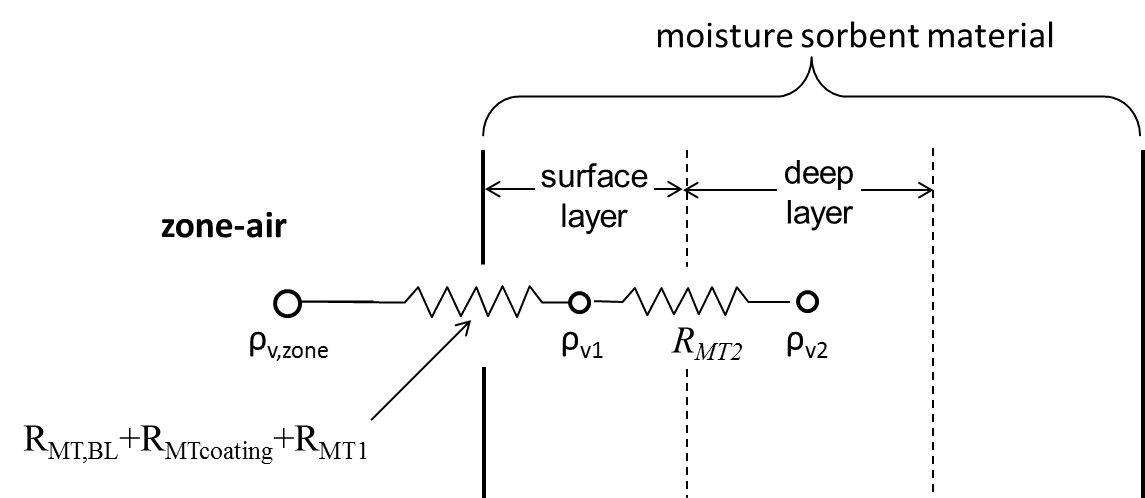
\includegraphics[width=0.9\textwidth, height=0.9\textheight, keepaspectratio=true]{media/EMPDschematic.png}
\caption{Nodal network for effective moisture pentration depth model \protect \label{fig:Nodal-network-for-effective-moisture-penetration-depth-model}}
\end{figure}

The surface layer resistance is calculated with:

\begin{equation}
R_{MT,1} = \frac{d_{EMPD,1}} {2 \bar R_{water} T \delta_{perm}}
\end{equation}

where

\(d_{EMPD,1}\) = depth of surface layer, m

\(\bar R_{water}\) = universal gas constant for water (461.52 J/kg-K)

\(T\) = temperature, K

\(\delta_{perm}\) = water vapor permeability of the material, kg/m-s-Pa

The coating resistance is:

\begin{equation}
R_{MT,coating} = \frac {t_{coating} P_{ambient}} {\delta_{perm,coating} \bar R_{water} T}
\end{equation}

where

\(t_{coating}\) = coating thickness, m

\(P_{ambient}\) = ambient pressure, Pa

\(\delta_{perm,coating}\) = permeability of the coating, kg/m-s-Pa.

Finally, the boundary layer mass-transfer resistance is calculated by converting the heat-transfer coefficient to mass transfer with the Lewis relation:

\begin{equation}
R_{MT,BL} = \frac{\rho_{air} Cp_{air}}{h_{conv}}
\end{equation}

Behind the surface layer is a deep layer (labeled with subscipt 2 below) of thickness \(d_{EMPD,2}\). The surface layer accounts for buffering of high-frequency changes in the zone air humidity, while the deep layer accounts for the material's response to longer term changes in the zone air humidity. The model calculates the moisture flux between the surface and deep layers with:

\begin{equation}
j_{2} = \frac {\rho_{v,1} - \rho_{v,2}} {R_{MT,2}}
\end{equation}

where \(R_{MT,2}\) is:

\begin{equation}
R_{MT,2} = \frac {d_{EMPD,1} + d_{EMPD,2}} {2 \bar R_{water} T \delta_{perm} }
\end{equation}

These moisture fluxes are used to update the moisture content (or equivalent RH, \(\phi\) of each layer:

\begin{equation}
\phi_{1}(t) = \phi_{1}(t-\delta t) - \frac { (j_{zone} + j_{2}) \cdot TimeStep} {\rho_{matl} d_{EMPD,2} \frac {du}{d\phi}}
\end{equation}

\begin{equation}
\phi_{2}(t) = \phi_{2}(t-\delta t) + \frac { j_{2} \cdot TimeStep} {\rho_{matl} d_{EMPD,2} \frac {du}{d\phi}}
\end{equation}

where

$\rho_{matl}$ = Material dry density, $kg/m^3$

$TimeStep$ = Simulation timestep, s

$\frac {du}{d\phi}$ = slope of moisture curve (change in moisture content / change in RH), kg/kg $\cdot$ RH

The equivalent RH and equivalent vapor density are related with:

\begin{equation}
\rho_{v,1} = \frac {\phi_{1} P_{sat}(T)} {\bar R_{water}}
\end{equation}

\begin{equation}
\rho_{v,2} = \frac {\phi_{2} P_{sat}(T)} {\bar R_{water}}
\end{equation}

The zone flux is used, along with the area of the particular surface, to update the zone humidity ratio, as discussed in \ref{moisture-predictor-corrector}.

The zone flux is also used to calculate the sensible heat released (during adsorption) or absorbed (during desorption) at the material surface:

\begin{equation}
Q_{flux} = j_{zone} h_{fg}
\end{equation}

where \(h_{fg}\) is the enthalpy of vaporization of water, assumed to be 2500 kJ/kg. This is added to the heat balance calculations at the interior surface.

For further information on the EMPD model, see References below.

\subsection{EMPD Nomenclature}\label{empd-nomenclature}
\begin{align*}  
  A  &= \text{surface area} \RB{m^{2}} \\
  d &= \text{penetration depth} \RB{m} \\
  j &= \text{water mass flux} \RB{\frac{kg}{m^{2} \cdot s}} \\
  \bar R_{water} &= \text{universal gas constant for water,} \; 452.61 \RB{\frac{J}{kg \cdot K}}   \\
  R_{MT} &= \text{Mass transfer resistance} \RB{s/m} \\
  T &= \text{temperature} \RB{K} \\
  u &= \text{moisture content} \RB{\frac{kg}{kg}}
\end{align*}

\subsubsection{Greek letters}\label{greek-letters}
\begin{align*}  
  \delta  &= \text{permeability} \RB{\frac{kg}{m \cdot s \cdot Pa}} \\
  \phi &= \text{relative humidity} \\
  \rho &= \text{density} \RB{\frac{kg}{m^{3}}} \\
  \rho_{v} &= \text{vapor density} \RB{\frac{kg}{m^{3}}} \\
\end{align*}

\subsubsection{Subscripts}\label{subscripts-and-superscripts}
\begin{align*}
	1 &= \text{surface layer node} \\
	2 &= \text{deep layer node} \\
	BL &= \text{boundary layer} \\
	matl &= \text{solid material} \\
	zone &= \text{zone air} \\
\end{align*}

\subsection{References}\label{references-019}

Cunningham, M.J.,
\href{http://www.sciencedirect.com/science/article/pii/0360132388900261}{\emph{The
		moisture performance of framed structures - a mathematical model}},
Build. Environ. 23 (1988) 123-35.

Kerestecioglu, A., M. Swami, R. Dabir, N. Razzaq, P. Fairey,
\href{http://www.fsec.ucf.edu/en/publications/pdf/FSEC-CR-191-88.pdf}{\emph{Theoretical
		and Computational Investigation of Algorithms for Simultaneous Heat and
		Moisture Transport in Buildings}}. Florida Solar Energy Center,
DOE/SF/16305-2, 1988.

Cunningham, M.J.,
\href{http://www.sciencedirect.com/science/article/pii/036013239290037P}{\emph{Effective
		penetration depth and effective resistance in moisture transfer}},
Build. Environ. 27 (1992) 379-86

Janssen, H. and S. Roels,
\href{http://www.sciencedirect.com/science/article/pii/S0378778808002387}{\emph{Qualitative
		and quantitative assessment of interior moisture buffering by
		enclosures}}, Energ. Buildings. 41 (2009) 382-94.

Abadie, M.O. and K.C. Mendonca,
\href{http://www.sciencedirect.com/science/article/pii/S0360132308000528}{\emph{Moisture
		performance of building materials: From material characterization to
		building simulation using the Moisture Buffer Value concept}}, Build.
Environ. 44 (2009) 388-401.

Vereecken, E., S. Roels, H. Janssen,
\href{http://jen.sagepub.com/content/34/3/223.abstract}{\emph{In situ
		determination of the moisture buffer potential of room enclosures}}, J.
Build. Phys. 34 (2011) 223-46.

Woods, J., Winkler, J, and Christensen, D.
\href{http://www.nrel.gov/docs/fy13osti/57441.pdf}{\emph{Evaluation of
		the Effective Moisture Penetration Depth Model for Estimating Moisture
		Buffering in Buildings}}, NREL/TP-5500-57441, 2013.

Woods, J., J. Winkler, D. Christensen, E. Hancock,
\href{http://www.nrel.gov/docs/fy14osti/62456.pdf}{\emph{Using
		Whole-House Field Tests to Empirically Derive Moisture Buffering Model
		Inputs}}. NREL/TP-5500-62456, 2014.

